\documentclass{article}
\usepackage{tikz}
\usepackage{array}
\usetikzlibrary{shapes.geometric, arrows}

\tikzstyle{startstop} = [rectangle, rounded corners, minimum width=3cm, minimum height=1cm,text centered, draw=black, fill=red!30]
\tikzstyle{io} = [trapezium, trapezium left angle=70, trapezium right angle=110, minimum width=3cm, minimum height=1cm, text centered, draw=black, fill=blue!30, text width = 2cm]
\tikzstyle{process} = [rectangle, minimum width=3cm, minimum height=1cm, text centered, draw=black, fill=orange!30, text width = 2cm]
\tikzstyle{decision} = [diamond, minimum width=3cm, minimum height=1cm, text centered, draw=black, fill=green!30, text width = 2cm]
\tikzstyle{arrow} = [thick,->,>=stealth]

\begin{document}
\title{XSGen}
\date{January, 25, 2017}
\author{Flanagan, Robert \and Scopatz, Anthony}
\maketitle

\section{Introduction}
As the development and deployment of new nuclear reactor technologies increases, the impacts of these technologies must be fully characterized. One possible avenue for accomplishing this is using fuel cycle simulators capable of representing the physics the occurs inside these reactors. Several simulators exist, but not all can model the physics internal to these reactors. Some that are capable of this level of physics are COSI [citation needed], CLASS [citation needed] and certain modules within Cyclus [citation needed]. 

Being able to model reactors accurately is important for moving nuclear fuel cycle design forward. A fuel cycle is primarily defined by the quality (composition) of materials that move through it. This primarily comes from the reliance of down stream facilities on the materials that are made available to them upstream. For example, the behavior and cost of a reprocessing facilities depends on the material that is made available to it by reactors. This behavior is unique to nuclear fuel as the composition of used materials can very greatly based on the physics of a facility. Developing increased medium fidelity models therefore leads to better understanding of the behavior of a nuclear fuel cycle. 

Bright-lite [citation needed] is a medium fidelity reactor model for Cyclus. It uses a fluence based approached to calculate appropriate discharge fluence, and isotopic vectors for a reactor. To accomplish this, it uses criticality, burnup, and transmutation matrices for each isotope of the reactors input fuel of a given reactor type. This information is generated using one group cross sections and a Bateman Equation solver. The reliance on one group cross sections means that the fidelity of the calculations is only as good as the data, and method, used to generate the one group cross sections. Therefore, improving the physics models used to generate the one group cross sections will improve the fidelity of the results generated by Bright-lite. 

There are several existing techniques for generating the required data for Bright-lite to operate. MCNP[MCNP citication] and Monteburns[citation required] are both software that are capable of producing results that Bright-lite could use, but both have flaws. MCNP is primilary a monte carlo code, it does however, have a fuel burning function (the burn card) within it. Unfortunately it does not provide all of the cross sections and reactions that Bright-lite is interested in. 

Monteburns functions very similar to the burn card currently in MCNP. It extracts cross sections from MCNP and uses those to create one group cross sections for a bateman equation solver, it then simulates burning the fuel. This is the ideal path for producing Bright-lite data, however, Monteburns is lacking in some very important charactistics. First, Monteburns is limited to the reactor types that are included with the software. This is problematic because Bright-lite aims to simulate newer and more advanced reactor types. Therefore, any software for linking into Bright-lite must be flexible in terms of reactor design. Second, Monteburns is not capable of producing multigroup cross sections. While Bright-lite is not capable of yet using multigroup cross sections, that is one goal of the software moving forward.   

XSGen is a new methodology aimed at developing higher accuracy cross sections. Similar to the work flow of Monteburns, it couples a Monte Carlo software with a Bateman Equation solver.  By coupling the two software it is possible to generate fluence dependent values for neutron production, destruction, and transmutation matrices for each isotope as the flux spectrum within a reactor evolves. It provides the capability to investigate any cross section that exists in ENDF, EAF, and ACE cross section databases, to collapse them into single or multigroup cross sections, and to provide the data required by Bright-lite directly. 

\section{XSGen Work Flow}
The XSGen work flow is composed of 3 main parts as mentioned above. The first step is the simulation of the reactor core using a Monte Carlo simulation. The results of this are then taken in by a wrapping software and converted into one group cross sections for a specific reactor. These cross sections are then used inside of the Bateman Equation software to calculation the burnup, neutron production, neutron destruction, and transmutation matrixes. This values are calculated at a user defined time length. The composition of the material at the end of the time step is then returned to the Monte Carlo simulator and the process is repeated.

\begin{center}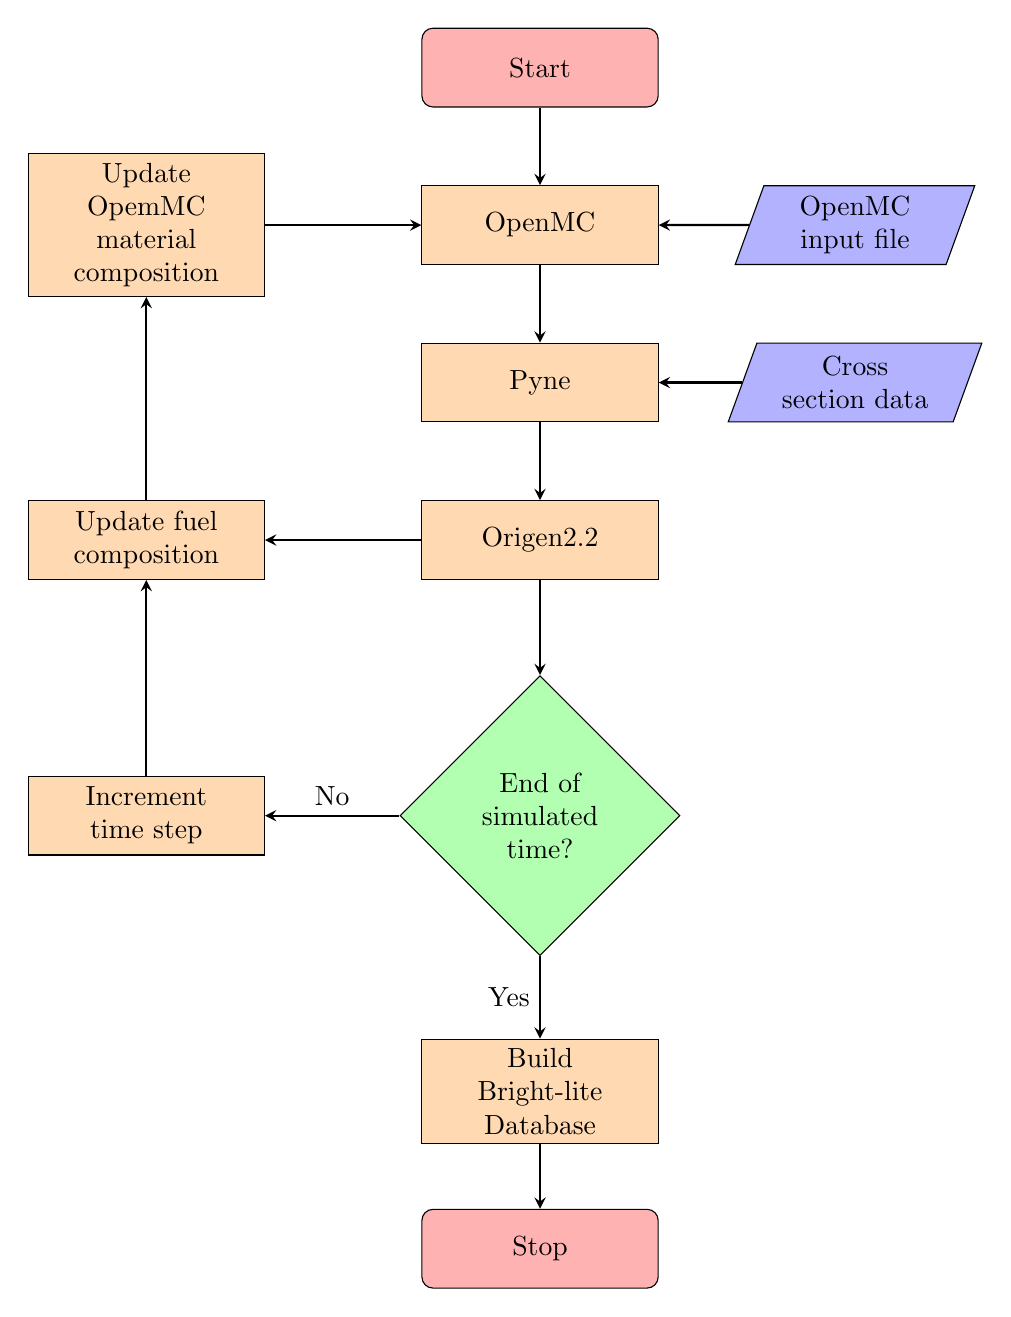
\begin{tikzpicture}[node distance=2cm]
\node (start) [startstop] {Start};
\node (openmc) [process, below of = start]{OpenMC};
\node (omcinput) [io, right of = openmc, xshift = 2cm]{OpenMC input file};
\node (omcupdate) [process, left of = openmc, xshift = -3cm]{Update OpemMC material composition};
\node (pyne) [process, below of = openmc]{Pyne};
\node (pynexs) [io, right of = pyne, xshift = 2cm]{Cross section data};
\node (origen22) [process, below of = pyne]{Origen2.2};
\node (compupdate) [process, left of = origen22, xshift = -3cm]{Update fuel composition};
\node (timecheck) [decision, below of = origen22, yshift = -1.5cm]{End of simulated time?};
\node (timeinc) [process, left of = timecheck, xshift = -3cm]{Increment time step};
\node (brightlite) [process, below of = timecheck, yshift = -1.5cm]{Build Bright-lite Database};
\node (stop) [startstop, below of = brightlite] {Stop};
\draw [arrow] (start) -- (openmc);
\draw [arrow] (omcinput) -- (openmc);
\draw [arrow] (omcupdate) -- (openmc);
\draw [arrow] (openmc) -- (pyne);
\draw [arrow] (pynexs) -- (pyne);
\draw [arrow] (pyne) -- (origen22);
\draw [arrow] (origen22) -- (timecheck);
\draw [arrow] (origen22) -- (compupdate);
\draw [arrow] (compupdate) -- (omcupdate);
\draw [arrow] (timeinc) -- (compupdate);
\draw [arrow] (timecheck) -- node[anchor=south]{No}(timeinc);
\draw [arrow] (timecheck) -- node[anchor=east]{Yes}(brightlite);
\draw [arrow] (brightlite) -- (stop);
\end{tikzpicture}\end{center}

\subsection{OpenMC}
The software chosen to perform the Monte Carlo operations was OpenMC [OpenMC citation].  OpenMC was chosen due to its open source nature and ability to quickly perform the calculation required. The only information required from the results of the OpenMC run is the group fluxes. These are used later to calculation one group cross sections. 

Input templates for OpenMC can be added to the XSGen system as need reactor types become available for modeling. 

\subsection{PyNE}
PyNE, or Python for Nuclear Engineering [PyNE citation], is the software used to perform the group collapse. The functionality to perform this group collapse was added to PyNE to facilitate the coupling of these two software. The collapse is performed using the following method. 

The first thing that is computed is a collection of weights used to represent the background cross section for each isotope is created. These weights are important because they allow the system to incorporate self-shielding behavior into the collapsed cross sections. These factors scale the one group cross section up or down depending on the density of the isotope represented by this cross section. The more delute a isotope is within a material composition, the lower the effective cross section of the isotope. This done using the following equation.

$$\omega_{y,n}=\frac{1}{\frac{(\sum_(X\neq Y)N^x * σ_(t,g)^x}{N^y}+\sigma_{t,g}^y}$$

Here all isotopes in the fuel are included in the set of X, and Y is the isotope in question. $N_y$ represents the number density of isotope Y, and $\sigma_{t,n}$ represents the total cross section of an isotope in a specific energy bin, n. Therefore $\omega$ represents a two-dimensional matrix of X (number of isotopes) by G (number of groups). The number in each entry of the matrix is the cross section weight for a specific isotope, in a specific energy group. These weights must be recalculated every time-step as the number densities of the isotopes in the fuel will charge as burnup increases. 

Note, that the cross sections used in this calculation must be provided by an outside source. PyNE is capable of reading in cross sections from several different cross section libraries including; ENDF, Cinder, EAF, and OpenMC. In this case the OpenMC cross sections were used. 

Next a partial energy matrix (PEM) is constructed. This maps a higher resolution group structures to lower resolution group structures. It does this by determining the contribution of each of the higher resolution energy groups into the lower resolution energy groups using a weighted sum. As this calculation can be computationally expensive it is only performed once per time step. 

PEM CALCULATION

For the current use case of XSGen this lower group structure is always a one group, however it is not limited to that. The PEM is also able to map lower energy groups into higher energy group structures, but that is also not used by XSGen.  

Once the PEM is constructed a collapsed flux is generated. Again, this collapses a detailed group structure into a single group. 

$$\sigma_g = PEM ∙(\sigma*\omega)$$

Here, \begin{math}\phi\end{math} represents the vector of group fluxes, and $\phi_g$ is the collapsed flux. With the one group flux it is possible to generate the one group cross sections. 

$$\sigma_{i,g}^x=\frac{[PEM∙(\sigma_i^x*\phi*\omega)]}{\sigma_g} $$

Here $\sigma_{i,g}^x$ represents the one group cross section of specific type i, for isotope x. Once this has been completed for all the chosen isotopes and cross sections they are used to generate a TAPE9 cross section file for that time-step. 

\subsection{Origin2.2}
Once the TAPE9 has been constructed it is used to perform two types of burnup operations. The first burnup is performed on the fuel. This includes the full list of isotopes currently in the fuel. Once this burnup is performed the isotopic vector at the end of the fuel burn is passed back to OpenMC to start the operation all over again.  

The second type of burnup calculation is used to build a dataset for a specific isotope. These burnup runs take one kilogram of a pure isotope as the input fuel. At the end of the run, the burnup, neutron production/destruction, and transmutation matrix are all recorded. The isotopes of interest are chosen ahead of time by the user of the software, typically these are the isotopes that the user wishes to use as the input fuel for the reactor type/design that they are investigating. 

\section{Benchmarking}
\subsection{LWR Test Cases}
XSGen by itself can not directly be tested against operating reactor systems. It was originally designed to produce datasets a medium fidelity reactor model known as Bright-lite. Therefore, to benchmark XSGen it will be used in conjunction with Bright-lite to produce burnups and isotopes for several known reactor systems.  As Bright-lite has already been benchmarked several times using other datasets [BRIGHT-LITE Benchmark Citations] it is assumed that the operations within Bright-lite are accurate and any deviations within the results come from XSGen. 

The most well studied reactors in the world are light water reactors and as such these will be used as benchmarking tools for XSGen. Primarily the cases represent a range of different enrichments in several light water reactors, comparing the results from XSGen/Bright-lite to recipes from VISION. Additionally, the values will be tested against two cases modelling reactor startup behavior.  [vision citation / transition citation].

The XSGen/Bright-light will be benchmarked against VISION at 3.0, 3.5, 4.0, and 4.5 percent enrichment. Three batch cores will be assumed for all the enrichment test cases. 
The two cases being used to test XSGen in startup behavior will be a 3.1$\%$ enriched light water reactor using four batches and a 3.6$\%$ enriched light water reactor using four batches. The cases will be compared using burnups, isotopic composition of fresh and used fuel.

\subsection{Results}
\begin{table}[!htb]
\centering
\caption{A comparison of the output isotopics at equalibrium in the VISION fuel cycle simulator and the XSGen-Bright-lite system.}
\label{tab:a}
\begin{tabular}{c| c c c| c c c | c c c |}
 & \multicolumn{3}{c}{3.0\%} & \multicolumn{3}{c}{3.5\%} & \multicolumn{3}{c}{4.0\%} \\
Isotope & VISION & XSGen-BL & Diff & VISION & XSGen-BL & Diff & VISION & XSGen-BL & Diff \\
\hline
U235 & 6.75E-3 & 6.70E-03 & -0.78 & 6.80E-3 & 6.71E-3 & -1.30 & 6.95E-3 & 6.91E-3 & -0.562 \\
Pu238 & 1.23E-4 & 1.27E-4 & 3.01 & 1.85E-4 & 1.86E-4 & -0.41 & 2.52E-4 & 2.55E-4 & 1.35 \\
Pu239 & 5.15E-3 & 5.25E-3 & 1.95 & 5.41E-3 & 5.45E-3 & 0.66 & 5.64E-3 & 5.67E-3 & 0.57 \\
Pu240 & 2.38E-3 & 2.4E-3 & 0.97 & 2.60E-3 & 2.61E-3 & 0.25 & 2.78E-3 & 2.79E-3 & 0.4 \\
Pu241 & 1.30E-3 & 1.35E-3 & 3.69 & 1.48E-3 & 1.52E-3 & 2.74 & 1.62E-3 & 1.62E-3 & -0.02 \\
Pu242 & 5.43E-4 & 5.48E-4 & 0.88 & 6.92E-4 & 6.93E-4 & 0.10 & 8.17E-4 & 8.19E-04 & -0.28 \\
Am241 & 3.56E-5 & 3.86E-5 & 8.81 & 4.59E-5 & 5.17E-5 & 12.60 & 5.55E-5 & 6.04E-5 & 8.79 \\
Am243 & 9.38E-5 & 9.01E-5 & -3.94 & 1.37E-4 & 1.26E-4 & -7.47 & 1.76E-4 & 1.74E-4 & -1.40 \\
Cm242 & 1.38E-5 & 1.34E-5 & -3.19 & 1.88E-5 & 1.79E-5 & -4.91 & 2.33E-5 & 2.31E-5 & -0.83 \\
Cm244 & 2.79E-5 & 2.57E-5 & -7.94 & 4.38E-5 & 4.54E-5 & -6.06 & 7.06E-5 & 7.00E-5 & -0.90 \\
\hline
\end{tabular}
\end{table}

Table \ref{tab:a} shows a very strong agreement between VISION and Bright-light results using datasets created from light water reactors designed to these particular enrichments. Bright-light has been benchmarked [Bright-lite citations] against VISION previously using other datasets. This shows that given XSGen generated datasets allows for Bright-lite to match VISION to a 5\% tolence for a majority of isotopes. Those that exhibit the greatest deviations are high order transuranics. 

Am241 shows the largest deviations from the VISION data. There is more Am241 in every case than expected by the VISION results, and less of the species that are arise due to the presence of Am241; Am243, Cm242, Cm244. These results can be explained by a neutron absorption cross section error in Am241. If the neutron absorption cross section for Am241 is too low it can never transmute into Am242 and Am243, which in turn leads to an absence of curium isotopes. 

\begin{table}[!htb]
\centering
\caption{NEA core discharge data for a 3.1\% enriched light water reactor with startup behavior.}
\label{tab:b}
\begin{tabular}{lllll}
Batch & Burnup (MWd/kg) & U235 (\%) & Fissile Pu (\%) & Total Pu(\%) \\
1 & 12.04 & 0.64 & 0.464 & 0.633 \\
2 & 23.86 & 0.76 & 0.6 & 0.818 \\
3 & 31.75 & 0.8 & 0.677 & 0.921 \\
4 & 32.00 & 0.85 & 0.697 & 0.943 \\
Equil. & 33.00 & 0.85 & 0.688 & 0.943
\end{tabular}
\end{table}

\begin{table}[!htb]
\centering
\caption{The startup values and percent difference from the NEA data for the XSGen/Bright-lite reactor system.}
\label{tab:c}
\begin{tabular}{lllllllll}
 & \multicolumn{2}{l}{Burnup (MWd/kgIHM)} & \multicolumn{2}{l}{U235 (\%)} & \multicolumn{2}{l}{Fissile Pu (\%)} & \multicolumn{2}{l}{Total Pu (\%)} \\
Batch & Value & \%Diff & Value & \%Diff & Value & \%Diff & Value & \%Diff \\
1 & 13.570 & 12.754 & 0.656 & 2.50 & 0.550 & 18.737 & 0.680 & 7.541 \\
2 & 22.040 & -7.628 & 0.723 & -4.868 & 0.641 & 6.919 & 0.835 & 2.189 \\
3 & 32.510 & 2.394 & 0.789 & -1.375 & 0.710 & 4.883 & 0.970 & 5.231 \\
4 & 31.230 & -2.406 & 0.851 & 0.117 & 0.680 & -2.254 & 0.906 & -5.031 \\
5 & 33.010 & 0.030 & 0.843 & -0.824 & 0.703 & 2.198 & 0.946 & 0.285 \\
Equal. & 33.020 & 0.060 & 0.855 & 0.588 & 0.700 & 1.833 & 0.951 & 0.820
\end{tabular}
\end{table}

Table \ref{tab:b} shows how XSGen/Bright-lite compares to the NEA results. The equilibrium results here show good agreement with this case. As Bright-lite is often used to derive output isotopics from used fuels to be passed onto recycle scenarios, accurately predicting the equilibrium output isotopics is important. 

The results of the start up isotopics can be seen in Table \ref{tab:c}. There are some discrepencies in these results. First, the amount of plutonium generated within the first batch is significantly higher within Bright-lite compared to the NEA data. This trend only continues for the first two cycles. Due to the way Bright-lite operates, this is caused by the lower enriched batches within the startup core that do not have neutron poisons from fission products or other actinides. This means that there is a higher effective flux striking a high amount of U238 causing more generation of Pu239. The NEA benchmark has these low enrichment startup batches spread more evenly, Bright-lite has them all inside the inner most part of the circle. 

\begin{table}[!htb]
\centering
\caption{NEA data for a 3.6\% enriched light water reactor start up behavior.}
\label{tab:d}
\begin{tabular}{lllll}
Batch & Burnup (MWd/kg) & U235 (\%) & Fissile Pu (\%) & Total Pu(\%) \\
1 & 13.9 & 0.840 & 0.474 & 0.629 \\
2 & 22.67 & 0.721 & 0.642 & 0.892 \\
3 & 32.36 & 0.647 & 0.716 & 1.039 \\
4 & 41.00 & 0.640 & 0.785 & 1.177 \\
5 & 39.00 & 0.940 & 0.808 & 1.166 \\
6 & 40.60 & 0.88 & 0.817 & 1.194 \\
Equil. & 42.50 & 0.81 & 0..827 & 1.223
\end{tabular}
\end{table}

\begin{table}[!htb]
\centering
\caption{XSGen / Bright-lite data for the 3.6\% enriched light water reactor start up behavior.}
\label{tab:e}
\begin{tabular}{lllllllll}
 & \multicolumn{2}{l}{Burnup (MWd/kgIHM)} & \multicolumn{2}{l}{U235 (\%)} & \multicolumn{2}{l}{Fissile Pu (\%)} & \multicolumn{2}{l}{Total Pu (\%)} \\
Batch & Value & \%Diff & Value & \%Diff & Value & \%Diff & Value & \%Diff \\
1 & 13.37 & -3.84 & 0.930 & 10.77 & 0.62 & 30.43 & 0.78 & 23.53 \\
2 & 22.69 & 0.07 & 0.82 & 13.02 & 0.72 & 12.81 & 0.96 & 7.49 \\
3 & 32.38 & 0.03 & 0.72 & 11.08 & 0.78 & 8.46 & 1.07 & 2.69 \\
4 & 42.57 & 3.83 & 0.61 & -5.33 & 0.804 & 2.42 & 1.14 & -2.94 \\
5 & 41.00 & 5.13 & 0.85 & 9.526 & 0.79 & -2.81 & 1.10 & -5.91 \\
6 & 43.83 & 3.04 & 0.82 & 6.53 & 0.79 & -3.58 & 1.11 & -7.45 \\
Equal. & 42.32 & -0.43 & 0.81 & -0.44 & 0.79 & -4.54 & 1.11 & -9.42
\end{tabular}
\end{table}

Table \ref{tab:d} and Table \ref{tab:e} are repeats of Table {tab:b} and Table \ref{tab:c} for the 3.6$\%$ enriched light water reactor. Again, you see a similar trend in these two with the exception that the equilibrium results for the total amount of plutonium within the reactor is 9.2$\%$ lower in the Bright-lite model. The amount of fissile plutonium is also lower, but within acceptable bounds. The lower amount of fissile plutonium leads to less transmutations into the high order actinides. 

\section{MOX Case}
Simply replicating the behavior of a light water reactor would not show off the full capabilities of the XSGen software. To demonstrate the capability of the system to extend to more advanced reactor types, XSGen will be used to generate a MOX fuel library for Bright-lite. It will then be used to simulate a single pass MOX reactor. In order to compare this on an apples to apples basis, the input fuel into the Bright-lite reactor will be exactly the same as that for a similar VISION reactor. This test will be able to demonstrate the flexibility of the combined XSGen/Bright-lite system that allows it to model advanced reactor types. 

\begin{table}[!htb]
\centering
\caption{Comparison of VISION and Bright-lite result from a single pass MOX reactor.}
\label{tab:g}
\begin{tabular}{llllll}
Isotope & Input Composition & Vision & Bright-lite & Difference(\%) \\
U234 & 2.20E-4 & 2.11E-4 & 2.00E-4 & -5.0\\
U235 & 7.08E-3 & 4.05E-3 & 4.00E-3 & -1.2\\
U236 & 5.28E-3 & 4.97E-3 & 5.60E-3 & 12.6\\
U238 & 8.80E-1 & 8.51E-1 & 8.62E-1 & 1.3\\
Pu238 & 2.85E-3 & 3.22E-3 & 3.01E-3 & -6.5\\
Pu239 & 5.66E-2 & 3.31E-2 & 3.15E-2 & -4.6\\ 
Pu240 & 2.70E-2 & 2.42E-2 & 2.54E-2 & 5.0\\
Pu241 & 1.17E-2 & 1.31E-2 & 1.27E-2 & -3.3\\
Pu242 & 8.00E-3 & 8.90E-3 & 8.68E-3 & -2.6\\
Am241 & 1.18E-3 & 1.72E-3 & 1.60E-3 & -7.2\\
Am243 & - & 1.96E-3 & 1.83E-3 & -6.6\\
Cm242 & - & 2.62E-4 & 2.46E-4 & -6.4\\
CM244 & - & 1.03E-3 & 9.84E-4 & -4.4
\end{tabular}
\end{table}

The data in Table \ref{tab:g} shows that the results of Bright-lite given the new XSGen MOX reactor cross section fairs quite well compared to VISION. There are some outliers in the behaviors, specifically the higher order species and U236. 

One of the possible primary causes of this is uncertainity in the exact dimensions and behavior of the VISION MOX reactor. In order to get the most accurate results XSGen needs to know the specification of the MOX reactor. Instead for this result a generic 17x17 MOX core was chosen. 

\end{document}

